\chapter{Implementation}

\section{Installing new gateways in Furtwangen}

\section{A, B and C buildings}

\begin{figure}[h]
    \centering
    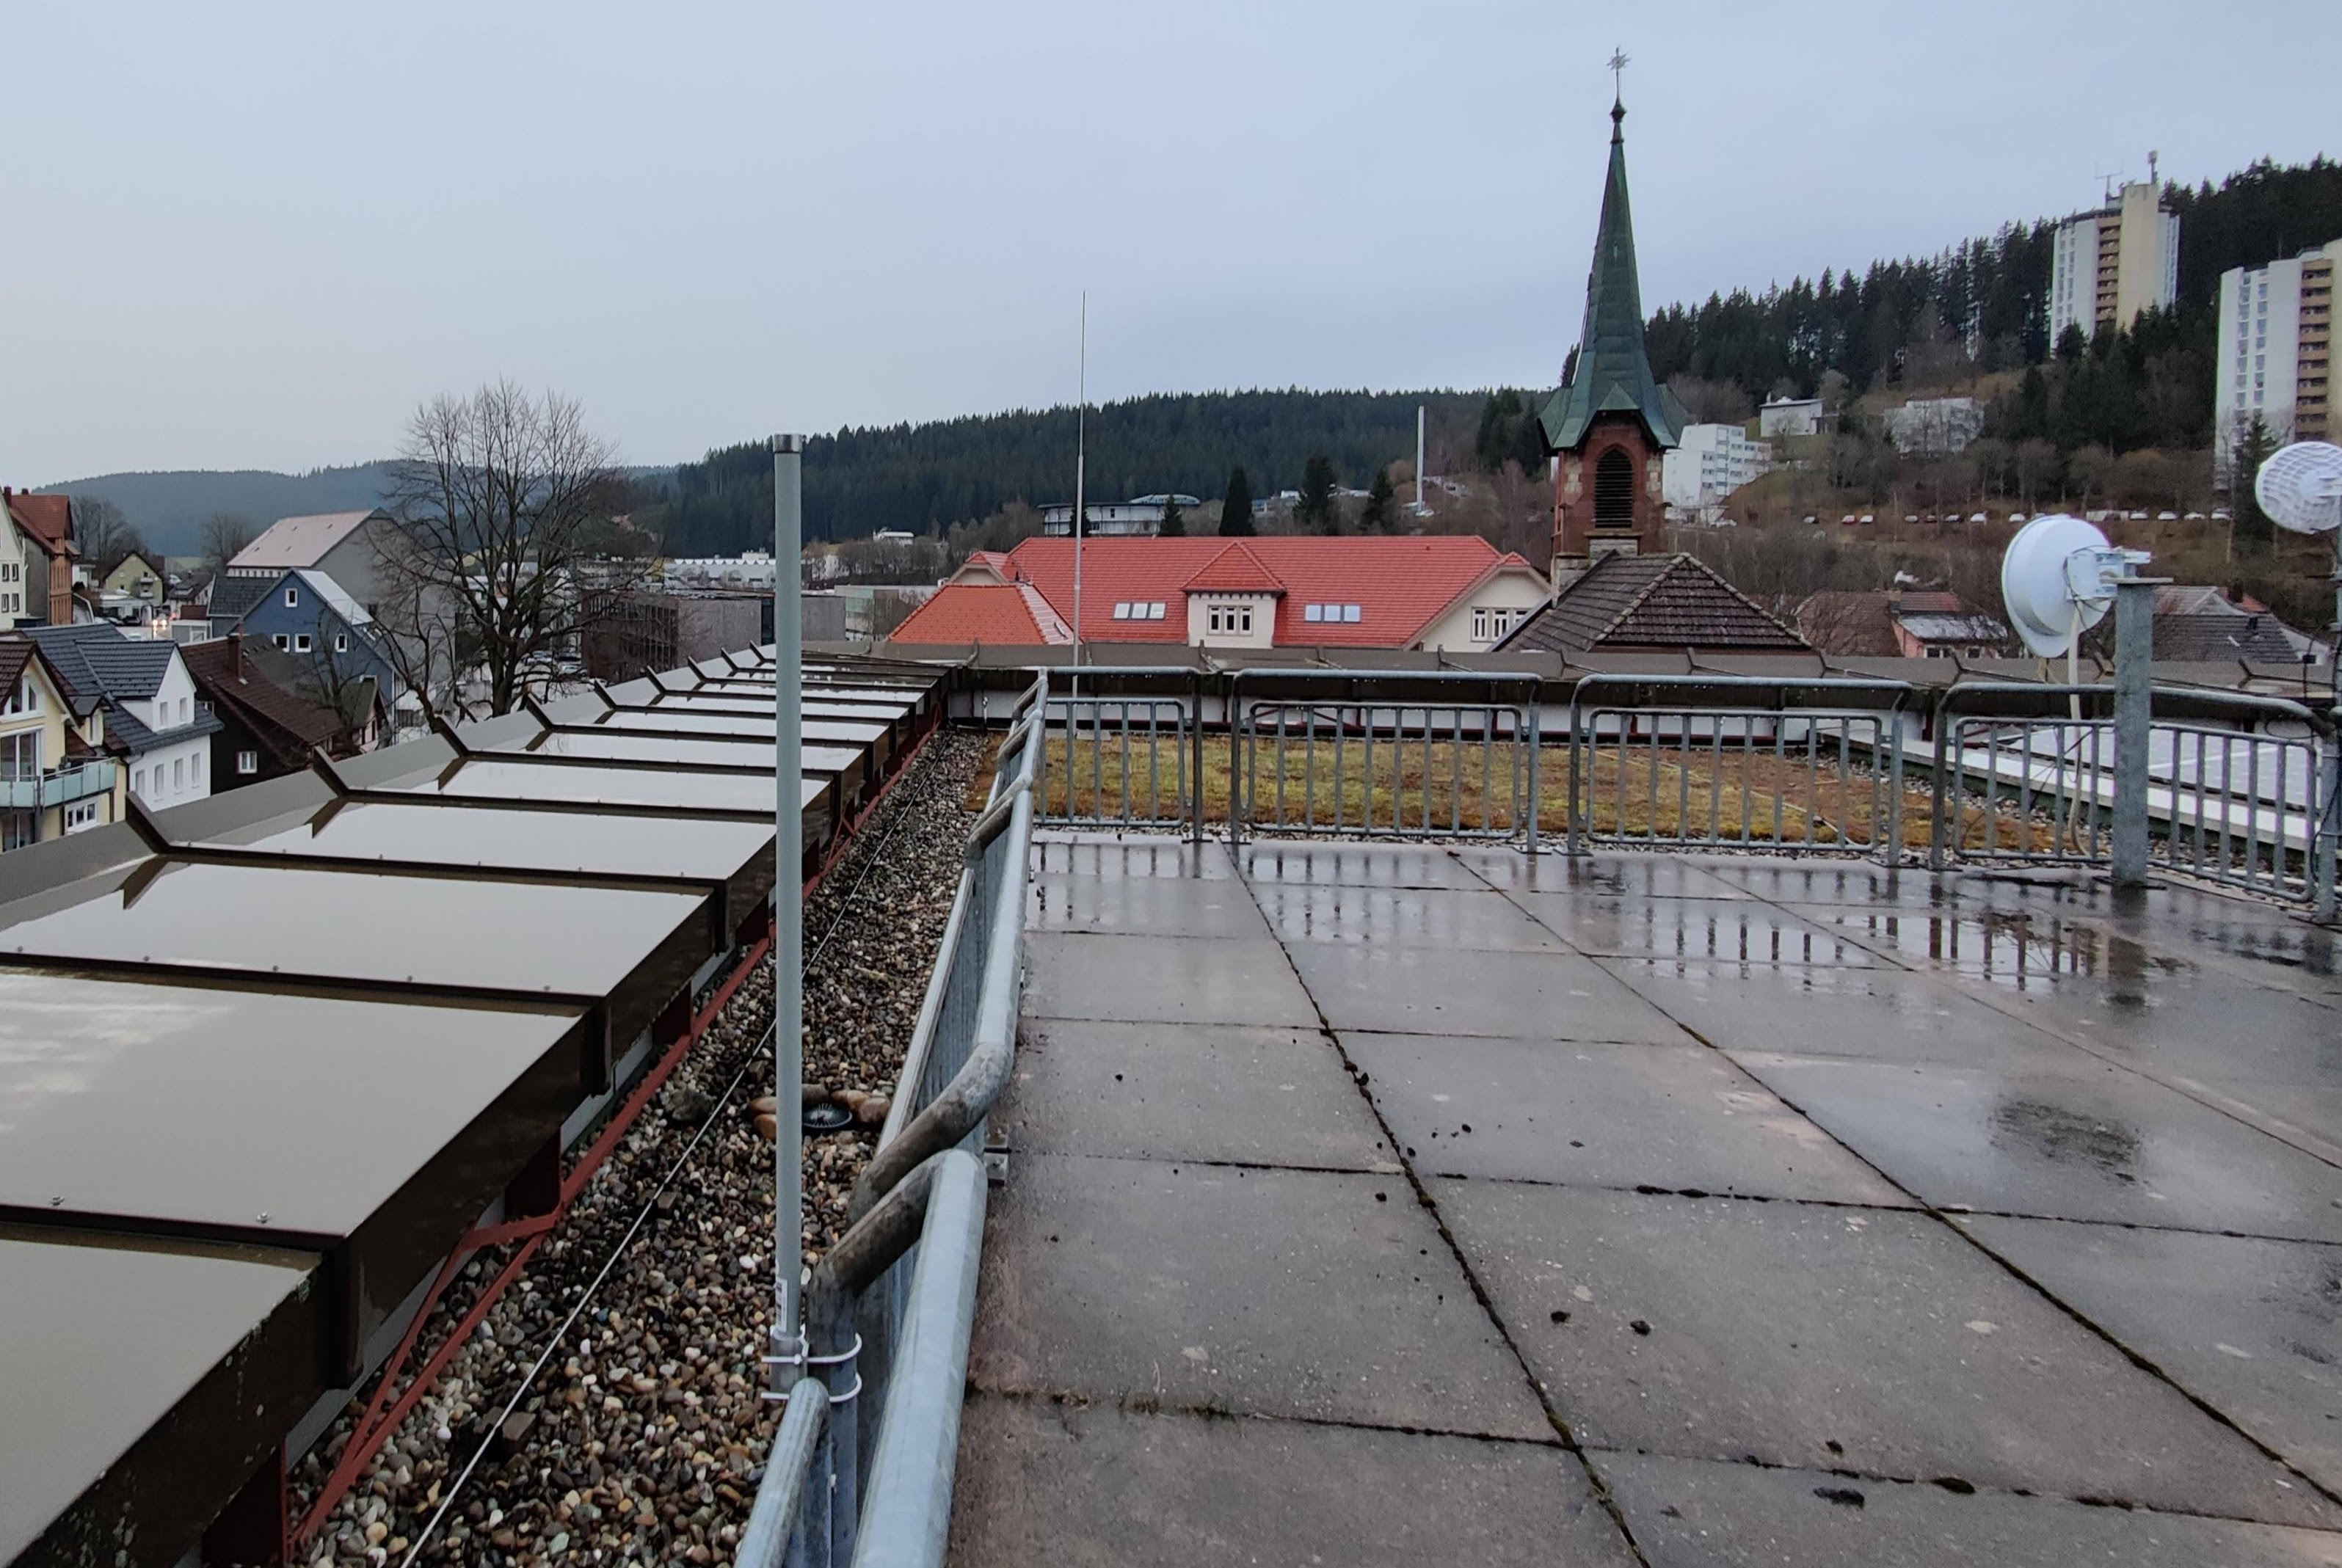
\includegraphics[width=0.6\textwidth]{pictures/hardware/gateway-deployment/mikrotik-antenna-c-building.jpg}
    \caption{The MikroTik antenna installed on top of the \ac{HFU} C building}\label{pic:mikrotik-antenna-c-building}
\end{figure}

The first antenna and gateway installed to last was the MikroTik antenna on top of the \ac{HFU} C building as seen in \cref{pic:mikrotik-antenna-c-building}.
While not as high in altitude as the GHB building, it is still a good location to receive signals from the surrounding area.

% ggf abbreviations?
\subsection{Großhausberg (GHB) and Albert-Schweizer-Haus (ASH) dormitories}

\subsection{Brend tower}

\section{Comparison of Geolocation Methods}

\section{Program structure}